%%
%% Automatically generated file from DocOnce source
%% (https://github.com/hplgit/doconce/)
%%

% #define PREAMBLE

% #ifdef PREAMBLE
%-------------------- begin preamble ----------------------

\documentclass[%
oneside,                 % oneside: electronic viewing, twoside: printing
final,                   % draft: marks overfull hboxes, figures with paths
10pt]{article}

\listfiles               %  print all files needed to compile this document

\usepackage{relsize,makeidx,color,setspace,amsmath,amsfonts,amssymb}
\usepackage[table]{xcolor}
\usepackage{bm,ltablex,microtype}

\usepackage[pdftex]{graphicx}

\usepackage[T1]{fontenc}
%\usepackage[latin1]{inputenc}
\usepackage{ucs}
\usepackage[utf8x]{inputenc}

\usepackage{lmodern}         % Latin Modern fonts derived from Computer Modern

% Hyperlinks in PDF:
\definecolor{linkcolor}{rgb}{0,0,0.4}
\usepackage{hyperref}
\hypersetup{
    breaklinks=true,
    colorlinks=true,
    linkcolor=linkcolor,
    urlcolor=linkcolor,
    citecolor=black,
    filecolor=black,
    %filecolor=blue,
    pdfmenubar=true,
    pdftoolbar=true,
    bookmarksdepth=3   % Uncomment (and tweak) for PDF bookmarks with more levels than the TOC
    }
%\hyperbaseurl{}   % hyperlinks are relative to this root

\setcounter{tocdepth}{2}  % levels in table of contents

% Tricks for having figures close to where they are defined:
% 1. define less restrictive rules for where to put figures
\setcounter{topnumber}{2}
\setcounter{bottomnumber}{2}
\setcounter{totalnumber}{4}
\renewcommand{\topfraction}{0.95}
\renewcommand{\bottomfraction}{0.95}
\renewcommand{\textfraction}{0}
\renewcommand{\floatpagefraction}{0.75}
% floatpagefraction must always be less than topfraction!
% 2. ensure all figures are flushed before next section
\usepackage[section]{placeins}
% 3. enable begin{figure}[H] (often leads to ugly pagebreaks)
%\usepackage{float}\restylefloat{figure}

% newcommands for typesetting inline (doconce) comments
\newcommand{\shortinlinecomment}[3]{{\color{red}{\bf #1}: #2}}
\newcommand{\longinlinecomment}[3]{{\color{red}{\bf #1}: #2}}

\usepackage[framemethod=TikZ]{mdframed}

% --- begin definitions of admonition environments ---

% Admonition style "mdfbox" is an oval colored box based on mdframed
% "notice" admon
\definecolor{mdfbox_notice_background}{rgb}{1,1,1}
\newmdenv[
  skipabove=15pt,
  skipbelow=15pt,
  outerlinewidth=0,
  backgroundcolor=mdfbox_notice_background,
  linecolor=black,
  linewidth=2pt,       % frame thickness
  frametitlebackgroundcolor=mdfbox_notice_background,
  frametitlerule=true,
  frametitlefont=\normalfont\bfseries,
  shadow=false,        % frame shadow?
  shadowsize=11pt,
  leftmargin=0,
  rightmargin=0,
  roundcorner=5,
  needspace=0pt,
]{notice_mdfboxmdframed}

\newenvironment{notice_mdfboxadmon}[1][]{
\begin{notice_mdfboxmdframed}[frametitle=#1]
}
{
\end{notice_mdfboxmdframed}
}

% Admonition style "mdfbox" is an oval colored box based on mdframed
% "summary" admon
\definecolor{mdfbox_summary_background}{rgb}{1,1,1}
\newmdenv[
  skipabove=15pt,
  skipbelow=15pt,
  outerlinewidth=0,
  backgroundcolor=mdfbox_summary_background,
  linecolor=black,
  linewidth=2pt,       % frame thickness
  frametitlebackgroundcolor=mdfbox_summary_background,
  frametitlerule=true,
  frametitlefont=\normalfont\bfseries,
  shadow=false,        % frame shadow?
  shadowsize=11pt,
  leftmargin=0,
  rightmargin=0,
  roundcorner=5,
  needspace=0pt,
]{summary_mdfboxmdframed}

\newenvironment{summary_mdfboxadmon}[1][]{
\begin{summary_mdfboxmdframed}[frametitle=#1]
}
{
\end{summary_mdfboxmdframed}
}

% Admonition style "mdfbox" is an oval colored box based on mdframed
% "warning" admon
\definecolor{mdfbox_warning_background}{rgb}{1,1,1}
\newmdenv[
  skipabove=15pt,
  skipbelow=15pt,
  outerlinewidth=0,
  backgroundcolor=mdfbox_warning_background,
  linecolor=black,
  linewidth=2pt,       % frame thickness
  frametitlebackgroundcolor=mdfbox_warning_background,
  frametitlerule=true,
  frametitlefont=\normalfont\bfseries,
  shadow=false,        % frame shadow?
  shadowsize=11pt,
  leftmargin=0,
  rightmargin=0,
  roundcorner=5,
  needspace=0pt,
]{warning_mdfboxmdframed}

\newenvironment{warning_mdfboxadmon}[1][]{
\begin{warning_mdfboxmdframed}[frametitle=#1]
}
{
\end{warning_mdfboxmdframed}
}

% Admonition style "mdfbox" is an oval colored box based on mdframed
% "question" admon
\definecolor{mdfbox_question_background}{rgb}{1,1,1}
\newmdenv[
  skipabove=15pt,
  skipbelow=15pt,
  outerlinewidth=0,
  backgroundcolor=mdfbox_question_background,
  linecolor=black,
  linewidth=2pt,       % frame thickness
  frametitlebackgroundcolor=mdfbox_question_background,
  frametitlerule=true,
  frametitlefont=\normalfont\bfseries,
  shadow=false,        % frame shadow?
  shadowsize=11pt,
  leftmargin=0,
  rightmargin=0,
  roundcorner=5,
  needspace=0pt,
]{question_mdfboxmdframed}

\newenvironment{question_mdfboxadmon}[1][]{
\begin{question_mdfboxmdframed}[frametitle=#1]
}
{
\end{question_mdfboxmdframed}
}

% Admonition style "mdfbox" is an oval colored box based on mdframed
% "block" admon
\definecolor{mdfbox_block_background}{rgb}{1,1,1}
\newmdenv[
  skipabove=15pt,
  skipbelow=15pt,
  outerlinewidth=0,
  backgroundcolor=mdfbox_block_background,
  linecolor=black,
  linewidth=2pt,       % frame thickness
  frametitlebackgroundcolor=mdfbox_block_background,
  frametitlerule=true,
  frametitlefont=\normalfont\bfseries,
  shadow=false,        % frame shadow?
  shadowsize=11pt,
  leftmargin=0,
  rightmargin=0,
  roundcorner=5,
  needspace=0pt,
]{block_mdfboxmdframed}

\newenvironment{block_mdfboxadmon}[1][]{
\begin{block_mdfboxmdframed}[frametitle=#1]
}
{
\end{block_mdfboxmdframed}
}

% --- end of definitions of admonition environments ---

% prevent orhpans and widows
\clubpenalty = 10000
\widowpenalty = 10000

% --- end of standard preamble for documents ---


\usepackage[swedish]{babel}

\raggedbottom
\makeindex
\usepackage[totoc]{idxlayout}   % for index in the toc
\usepackage[nottoc]{tocbibind}  % for references/bibliography in the toc

%-------------------- end preamble ----------------------

\begin{document}

% matching end for #ifdef PREAMBLE
% #endif

\newcommand{\exercisesection}[1]{\subsection*{#1}}

% This file is to be run by preprocess to produce newcommands.tex
% to be included in .tex files.
% There are format-specific tests here for the newcommands (i.e.,
% different definitions of the commands depending on latex or mathjax).

% Newcommands for LaTeX math.
\newcommand{\tp}{\thinspace .}
\renewcommand{\Re}{\bbbr}
\newcommand{\Oof}[1]{\mathcal{O}(#1)}
\newcommand{\Prob}[1]{\hbox{P}(#1)}
\newcommand{\Var}[1]{\hbox{Var}(#1)}
\newcommand{\Cov}[2]{\hbox{Cov}(#1,#2)}
\newcommand{\StDev}[1]{\hbox{StDev}(#1)}

\newcommand{\punkt}{\thinspace .}
\newcommand{\komma}{\thinspace ,}

\newcommand{\vr}{\vec{r}}
\newcommand{\vrp}{\vec{r}\,'}
\newcommand{\erf}{\mathrm{erf}}
\newcommand{\vrho}{\vec{\varrho}}
\newcommand{\vrhop}{\vec{\varrho}\, '}
\newcommand{\sign}{\mathrm{sign}}

\newcommand{\Tr}[1]{\mathrm{Tr}[#1]}
\newcommand{\e}{\varepsilon}
\newcommand{\g}{\gamma}

\newcommand{\half}{\frac{1}{2}}
\newcommand{\vnabla}{\vec{\nabla}}


% Use footnotesize in subscripts
\newcommand{\subsc}[2]{#1_{\mbox{\footnotesize #2}}}




% ------------------- main content ----------------------



% ----------------- title -------------------------

\thispagestyle{empty}

\begin{center}
{\LARGE\bf
\begin{spacing}{1.25}
FFM234, Klassisk fysik och vektorfält - Föreläsningsanteckningar
\end{spacing}
}
\end{center}

% ----------------- author(s) -------------------------

\begin{center}
{\bf \href{{http://fy.chalmers.se/subatom/tsp/}}{Christian Forssén}, Institutionen för fysik, Chalmers, Göteborg, Sverige${}^{}$} \\ [0mm]
\end{center}

\begin{center}
% List of all institutions:
\end{center}
    
% ----------------- end author(s) -------------------------

% --- begin date ---
\begin{center}
Aug 18, 2020
\end{center}
% --- end date ---

\vspace{1cm}


\section*{9. Lösningar av Poissons ekvation}
Vi vet att Poissons ekvation
$$
\Delta \phi(\vec{r}) = - \rho(\vec{r}),
$$
har entydiga lösningar om
\begin{align}
\phi|_{\partial V} &= f(\vec{r}) \quad & \mathrm{Dirichlets~randvillkor} \nonumber \\
(\vnabla\phi)|_{\partial V} \cdot \vec{n} &= g(\vec{r}) \quad & \mathrm{Neumans~randvillkor} \nonumber 
\end{align}
där $f$ och $g$ är funktioner på randen $\partial V$.


\begin{summary_mdfboxadmon}[Lösning av Poissons ekvation]
Vi kommer att betrakta fyra olika lösningsmetoder:

\paragraph{1. Greensfunktionsmetoden.}
Generell metod, men det är ofta svårt att finna analytiska uttryck för Greensfunktionen.
\paragraph{2. Spegling.}
Ger uttryck för Greensfunktionen i vissa speciella geometrier och homogena randvillkor.
\paragraph{3. Variabelseparation.}
Kraftfull analytisk metod. Riktigt användbar i kombination med Fourieranalys.
\paragraph{4. Numeriska metoder.}
\begin{itemize}
\item De tre förstnämnda är analytiska metoder som vi introducerar för att ge en fysikalisk förståelse av lösningarna.

\item De numeriska metoderna är förstås viktigast för praktiska tillämpningar. Se datoruppgift.
\end{itemize}

\noindent
\end{summary_mdfboxadmon} % title: Lösning av Poissons ekvation



\subsection*{3. Variabelseparation}

\begin{itemize}
\item Bygger på att man löser ekvationerna stegvis för en variabel i taget. 

\item Problemet skall \emph{passa bra} ihop med ett visst koordinatsystem.
\end{itemize}

\noindent

\begin{notice_mdfboxadmon}[Exempel: Laplaces ekvation på en cirkelskiva]
\begin{itemize}
\item $\Delta\phi=0$, på $\varrho=\sqrt{x^2+y^2}<a$. 

\item Betrakta fallet där randvillkoret enbart innehåller ett vinkelberoende
\end{itemize}

\noindent
$$
\left. \phi(\vec{r}) \right|_{\partial V} = h(\varphi)
$$

Laplaceoperatorn är
$$
\Delta = \frac{1}{\varrho} \frac{\partial}{\partial \varrho} \varrho \frac{\partial}{\partial \varrho} +
 \frac{1}{\varrho^2} \frac{\partial^2}{\partial \varphi^2}.
$$
Målet är att lösa ekvationen, samtidigt som vi uppfyller randvillkoret, genom att separera beroendet på variabeln $\varphi$ och $\varrho$ genom en ansats av formen
$$
\phi(\varrho,\varphi) = f(\varrho) g(\varphi)
$$

\paragraph{Exempel.}
Antag att randvillkoret är
$$
\phi(a,\varphi)=\phi_0\cos m\varphi,
$$ 
där $m$ är ett heltal.

Vi ansätter att hela lösningen har just detta beroende av $\varphi$, så att 
$$
\phi(\varrho,\varphi)=f(\varrho)\cos m\varphi
$$
Funktionen $\cos m\varphi$ uppfyller 
$$
\frac{\partial ^2}{\partial \varphi^2} \cos m\varphi = -m^2 \cos m\varphi,
$$
dvs, den är en egenfunktion till $\frac{\partial^2}{\partial \varphi^2}$ med egenvärdet $-m^2$. 

Insättning:
$$
\frac{1}{\varrho} \frac{\mbox{d}}{\mbox{d}\varrho} \left( \varrho \frac{\mbox{d}f(\varrho)}{\mbox{d}\varrho} \right) \cos m \varphi - \frac{m^2}{\varrho^2}f(\varrho)\cos m\varphi=0,
$$
och om detta skall gälla överallt på cirkelskivan måste man ha
$$
\varrho \frac{\mbox{d}}{\mbox{d}\varrho} \left(\varrho \frac{\mbox{d}f(\varrho)}{\mbox{d}\varrho} \right)
-m^2f(\varrho)=0.
$$
Den partiella differentialekvationen har nu reducerats till en ordinär differentialekvation för funktionen $f(\varrho)$

\begin{itemize}
\item Ansatz: $f(\varrho)=A\varrho^p$ 

\item Löser ekvationen med $p^2-m^2=0$, dvs.~$p=\pm m$, där minustecknet väljs bort på grund av singulariteten i origo. 

\item Slutsats:
\end{itemize}

\noindent
$$
\phi(\varrho,\varphi)=\phi_0\left( \frac{\varrho}{a}\right)^m \cos m\varphi,
$$
är en lösning till Laplaces ekvation på cirkelskivan med randvillkoret $\phi(a,\varphi)=\phi_0\cos m\varphi$.
\end{notice_mdfboxadmon} % title: Exempel: Laplaces ekvation på en cirkelskiva




\begin{notice_mdfboxadmon}[Exempel 2: Laplaces ekvation på en cirkelskiva med allmänt Dirichlet randvillkor]


\begin{warning_mdfboxadmon}[OBS!]
Detta exempel inkluderar Fourieranalys som ej ingår i kursen. Anteckningarna är endast med för bättre koppling till motsvarande material i andra kurser och för att antyda den mer generella användningen av variabelseparationsmetoden.
\end{warning_mdfboxadmon} % title: OBS!



Med randvillkoret
$$
\phi(a,\varphi)=h(\varphi),
$$
ansätter vi lösningen $\phi(\varrho,\varphi) = f(\varrho) g(\varphi)$.

Laplacianen blir
$$
\Delta \phi = \Delta \left( f(\varrho) g(\varphi) \right) = g(\varphi) \frac{1}{\varrho} \frac{\partial}{\partial\varrho} \left( \varrho \frac{\partial f(\varrho)}{\partial\varrho} \right) + \frac{f(\varrho)}{\rho^2} \frac{\partial^2 g}{\partial\varphi^2} = 0.
$$
Detta ger den \emph{separerade} ekvationen
$$
\frac{f(\varrho) g(\varphi)}{\varrho^2} \left[ \frac{\varrho^2}{f(\varrho)} \frac{1}{\varrho} \frac{\partial}{\partial\varrho} \left( \varrho \frac{\partial f(\varrho)}{\partial\varrho} \right) + \frac{1}{g(\varphi)} \frac{\partial^2 g}{\partial\varphi^2} \right] = 0,
$$
där den första termen i hakparantesen enbart beror på $\varrho$ och den andra bara på $\varphi$. Därmed måste bägge vara konstanta (för att gälla för alla $\varrho,\varphi$). Vi sätter den första till $-\lambda$ och den andra till $+\lambda$.

Studera vinkelekvationen först
$$
\frac{\partial^2 g}{\partial\varphi^2} = \lambda g(\varphi),
$$
dvs vi kan tolka $g$ som en egenfunktion till $\partial^2 / \partial\varphi^2$. Lösningen är
$$
g(\varphi) = A \cos (m \varphi) + B \sin (m \varphi),
$$
med \emph{egenvärdet} $\lambda = -m^2$. Funktionen måste uppfylla randvillkoret $g(0) = g(2\pi)$ vilket ger att $m = 0,1,2,\ldots$ (notera att $m=0$ är meningslös för sinus-termen).

Den kvarvarande, radiella ekvationen blir nu
$$
\frac{1}{\varrho} \frac{\partial}{\partial\varrho} \left( \varrho \frac{\partial f(\varrho)}{\partial\varrho} \right) - \frac{m^2}{\varrho^2} f(\varrho) = 0.
$$

\begin{itemize}
\item $m=0$, vilket innebär att $g(\varphi) = A$
\end{itemize}

\noindent
$$
\frac{\partial}{\partial\varrho} \left( \varrho \frac{\partial f(\varrho)}{\partial\varrho} \right) = 0 \quad \Rightarrow \quad
\varrho \frac{\partial f(\varrho)}{\partial\varrho} = B \quad \Rightarrow \quad
\frac{\partial f(\varrho)}{\partial\varrho} = B \varrho.
$$
Med lösningen $f(\varrho) = A + B \ln(\varrho)$, där den andra termen motsvarar en punktkälla i två dimensioner (vi skippar denna).

Alltså är $\phi(\vec{r}) = A$ (konstant) en lösning om randvillkoret är $h(\varphi) = A$ (konstant).

\begin{itemize}
\item $m > 0$, ansätt lösning $f(\varrho) = C \varrho^p$
\end{itemize}

\noindent
$$
\frac{1}{\varrho} \frac{\partial}{\partial\varrho} \left( \varrho \frac{\partial}{\partial\varrho} \varrho^p \right) - \frac{m^2}{\varrho^2} \varrho^p = 0 \quad \Rightarrow \quad p^2 \varrho^{p-2} - m^2 \varrho^{p-2} = 0 \quad \Rightarrow \quad 
p = \pm m
$$
Med lösningen $f(\varrho) = A \varrho^m + \frac{B}{\varrho^m}$, där den andra termen är singulär i origo (vi skippar denna).

Med randvillkoret från ovan $h(\varphi) = \cos m \varphi$, $f(a) = \phi_0$ får vi lösningen
$$
\phi(\vec{r}) = \phi_0 \left( \frac{\varrho}{a} \right)^m \cos m\varphi,
$$
som ovan.

För ett mer allmänt randvillkor kan man (Fourier)-utveckla
$$
h(\varphi) = \sum_{m=0}^\infty a_m \cos(m\varphi) + b_m \sin(m\varphi),
$$
vilket ger lösningen
$$
\phi(\vec{r}) = \sum_{m=0}^\infty a_m \left( \frac{\varrho}{a} \right)^m \cos(m\varphi) + b_m \left( \frac{\varrho}{a} \right)^m \sin(m\varphi).
$$
OBS: ingår ej i denna kurs att kunna göra en sådan Fourierutveckling.
\end{notice_mdfboxadmon} % title: Exempel 2: Laplaces ekvation på en cirkelskiva med allmänt Dirichlet randvillkor




\begin{warning_mdfboxadmon}[Kommentar]
Separationsmetoden kan förstås användas med fler än två variabler. Vill man t.ex. använda den i sfäriska koordinater, hittar man egenfunktioner i tur och ordning i $\varphi$, $\theta$ och $r$. Se veckans tal. Eller så hittar man direkt egenfunktioner på $S^2$, s.k. klotytefunktioner (se kvantmekanik).
\end{warning_mdfboxadmon} % title: Kommentar



\subsection*{1. Greensfunktionsmetoden}

Vi tecknar Poissons ekvation i hela $\Bbb{R}^3$,
$$
\Delta\phi(\vec{r})=-\rho(\vec{r}).
$$ 
En lösningsstrategi som vi har betraktat tidigare är att:
\begin{itemize}
\item Beräkna bidraget till potentialen i punkten $\vec{r}$ givet en punktladdningen med styrkan $q=1$ belägen i punkten $\vec{r}\,'$.

\item Superpositionsprincipen ger potentialen som en summa/integral över källtätheten gånger ovanstående ``Greensfunktion''.
\end{itemize}

\noindent
Vi har redan visat att
$$
G_{\Bbb{R}^3}(\vec{r},\vec{r}{\;}') = \frac{1}{4\pi|\vec{r}-\vec{r}{\;}'|},
$$
där vi förtydligar att detta gäller på $\Bbb{R}^3$. Eftersom en punktkälla i punkten $\vec{r} = \vec{r}{\;}'$ med styrkan $q=1$ beskrivs av källtätheten $\rho(\vec{r}) = \delta^{(3)}(\vec{r} - \vec{r}{\;}')$, inser vi att Greensfunktionen löser följande differentialekvation
\begin{equation}
\Delta G_{\Bbb{R}^3}(\vec{r},\vec{r}{\;}') = -\delta^{(3)}(\vec{r} - \vec{r}{\;}'),
\label{eq:Greensdiffekv}
\end{equation}
på hela $\Bbb{R}^3$.

\longinlinecomment{Kommentar 1}{ Notera att Laplaceoperatorn verkar på variabeln $\vec{r}$ (inte $\vec{r}{\;}'$). Dvs., $\Delta = \Delta_{\vec{r}} = \partial_x^2 + \partial_y^2 + \partial_z^2$. }{ Notera att Laplaceoperatorn verkar }

Lösningen till Poissons ekvation i $\Bbb{R}^3$ med en allmän källa $\rho$ blir en superposition
$$
\phi(\vec{r})=\int_{\Bbb{R}^3}\mbox{d}V'\,\frac{\rho(\vec{r}{\;}')}{4\pi|\vec{r}-\vec{r}{\;}'|}.
$$


\begin{summary_mdfboxadmon}[Exempel: linjekälla]
Betrakta en linjekälla, $\rho(\vec{r})=k\delta^2(\vec{\rho})$, i $\Bbb{R}^3$.

Vi skall integrera över linjekällan och introducerar koordinaten
$$
\vec{r}{\;}' = \vec{\rho}{\;}' + z' \hat{z}' = \rho' \hat{\rho}' + z' \hat{z},
$$
där vi noterar att det inte behövs något ``prim'' på $z$-riktningen.

Vi sätter in i 
$$
\phi(\vec{r}) = \int_{\Bbb{R}^3}\rho(\vec{r}{\;}')G_{\Bbb{R}^3}(\vec{r},\vec{r}{\;}')\mbox{d}V'
=\int_{-\infty}^{\infty}dz'\int_{\Bbb{R}^2}dS'
       \frac{k\delta^2(\vec{\rho}{\;}')}{4\pi|\vec{r}-(\rho'\hat\rho{}'+z'\hat z)|} .
$$

Integralen $\int dS'$ över $x'$ och $y'$ kan enkelt utföras tack vare deltafunktionen. Resultatet:
$$
\phi(\vec{r})=\int_{-\infty}^{\infty}dz' \frac{k}{4\pi|\vec{r}-z'\hat z|}
$$  
som är identiskt med den direkta konstruktionen från kap. 6.
\end{summary_mdfboxadmon} % title: Exempel: linjekälla



\paragraph{Greensfunktioner för en begränsad volym med randvillkor.}
Låt oss göra denna metod mer generell. Studera Poissons ekvation 
$$
\Delta\phi(\vec{r})=-\rho(\vec{r}).
$$ 
\begin{itemize}
\item ... inuti en (begränsad) volym $V$.

\item ... med homogena randvillkor, dvs.~$f=0$ eller $g=0$ på randen $\partial V$.

\item ... för en allmän källtäthet $\rho(\vec{r})$.
\end{itemize}

\noindent
Lösningen kan skrivas
$$
\phi(\vec{r})=\int_{V'}\mbox{d}V'\,G(\vec{r},\vec{r}{\;}')\rho(\vec{r}{\;}'),
$$
där Greensfunktionen löser Ekv. (\ref{eq:Greensdiffekv}) \emph{inuti volymen} $V$ och med det \emph{givna randvillkoret}.

Att detta är en lösning visas genom insättning:
\begin{align}
\Delta\phi(\vec{r}) &= \Delta\int_{V'}\mbox{d}V'\,G(\vec{r},\vec{r}{\;}')\rho(\vec{r}{\;}')
=\int_{V'}\mbox{d}V'\,\Delta G(\vec{r},\vec{r}{\;}')\rho(\vec{r}{\;}') \nonumber \\
&=-\int_{V'}\mbox{d}V'\,\delta^3(\vec{r}-\vec{r}{\;}')\rho(\vec{r}{\;}')
=-\rho(\vec{r}).
\end{align}

\begin{itemize}
\item Notera att $\vec{r}$-beroendet bara sitter i Greensfunktionen.

\item Notera att Greensfunktionen $G$ på ett område $V$ bestäms av formen på området och av randvillkoren på $\partial V$.

\item Genom att $G(\vec{r},\vec{r}{\;}')$ uppfyller det homogena randvillkoret kommer ovanstående superposition också att uppfylla det.
\end{itemize}

\noindent
\subsection*{2. Spegling}

\begin{itemize}
\item Vi såg att lösningen $\phi(\vec{r})$ erhålls enkelt om man har tillgång till Greensfunktionen. Men denna är ofta svår att finna. 

\item För vissa geometrier erbjuder \emph{speglingsmetoden} ett väldigt elegant sätt att konstruera Greensfunktionen.
\end{itemize}

\noindent

\begin{summary_mdfboxadmon}[Rita: Fältbilder tre olika konfigurationer med punktladdningar]
Skissa fältbilder för tre olika fall:
\begin{itemize}
\item En punktladdning $+q$ (belägen i det övre halvplanet, $z>0$);

\item Två punktladdningar $+q$ och $-q$ (den första i det övre halvplanet och den andra i det undre);

\item Två punktladdningar $+q$ och $+q$ (den första i det övre halvplanet och den andra i det undre).
\end{itemize}

\noindent
Betrakta speciellt potentialen vid speglingsytan $z=0$.
\end{summary_mdfboxadmon} % title: Rita: Fältbilder tre olika konfigurationer med punktladdningar




\begin{summary_mdfboxadmon}[Fundera: Poissons ekvation]
Det första fallet ger en potential $\phi$ som löser Poissons ekvation 
$$
\Delta \phi = -q \delta^{(3)}(\vec{r}_0),
$$ 
i hela $\Bbb{R}^3$.
Vilken differentialekvation löser det andra respektive det tredje fallet om vi begränsar oss till övre halvplanet?
\end{summary_mdfboxadmon} % title: Fundera: Poissons ekvation



Betrakta halvrymden $\{\vec{r}:\,z>0\}$ med ett homogent randvillkor på planet
$z=0$: 
\begin{itemize}
\item Dirichlets randvillkor: $\phi=0$, eller 

\item Neumanns, $\frac{\partial \phi}{\partial z} = 0$.
\end{itemize}

\noindent
\longinlinecomment{Kommentar 2}{ Detta är ett bra tillfälle att repetera begreppen ekvipotentialytor och fältlinjer (till vektorfältet $-\vnabla\phi$). Se till att förstå att ett randvillkor $\phi=0$ (Dirichlet) betyder att randen är en ekvipotentialyta, och att $\vec n \cdot \vnabla\phi=0$ betyder att fältlinjerna är parallella med randen. }{ Detta är ett bra }

Betrakta nu en punktladdning belägen i det övre halvplanet. Vi kan införa en spegelladdning i det område som vi inte är intresserade av ($z<0$). Den påverkar alltså inte källtätheten i det fysikaliska området ($z>0$), men hjälper till att uppfylla randvillkoren.



\vspace{6mm}

% inline figure
\centerline{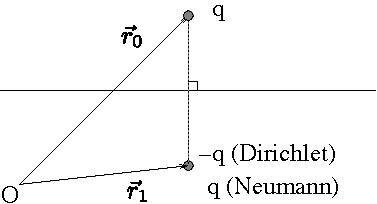
\includegraphics[width=0.5\linewidth]{fig/spegling.pdf}}

\vspace{6mm}



Med $\vec{r}_0 = (x_0,y_0,z_0)$ och $\vec{r}_1 = (x_0,y_0,-z_0)$ och:
\begin{itemize}
\item $q_1 = q$ uppfylls Neumanns randvillor

\item $q_1 = -q$ uppfylls Dirichlets randvillor
\end{itemize}

\noindent
dvs potentialen från den två punktladdningarna
$$
\phi(\vec{r}) = \frac{q}{4 \pi |\vec{r} - \vec{r}_0|} \pm \frac{q}{4 \pi |\vec{r} - \vec{r}_1|}
$$
I det förra fallet är fältlinjerna parallella med $z=0$ planet, i det senare fallet ligger ekvipotentialytan $\phi=0$ i $z=0$ planet.

Vi kan alltså konstruera Greensfunktioner för övre halvplanet med dessa två randvillkor. Med Dirichlets homogena randvillkor blir alltså Greensfunktionen
$$
G (\vec{r},\vec{r}\,')=\frac{1}{4\pi|\vec{r}-\vec{r}\,'|} - \frac{1} {4\pi|\vec{r}-\vec{r}\,''|},
$$
där $\vec{r}\,' = (x',y',z')$ och $\vec{r}\,'' = (x',y',-z')$, med $z'>0$.

Notera att $G(\vec{r},\vec{r}\,')$ uppfyller $\Delta G(\vec{r},\vec{r}\,') = - \delta(\vec{r}-\vec{r}\,')$ i det övre halvrummet.

Intressant nog fungerar speglingsmetoden även för cirklar i två dimensioner och sfärer i tre dimensioner (i det senare fallet dock endast för Dirichlets randvillkor). Se demonstrationsuppgift.



\vspace{6mm}

% inline figure
\centerline{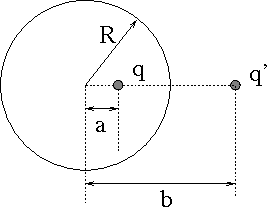
\includegraphics[width=0.5\linewidth]{fig/spegling2.pdf}}

\vspace{6mm}




% ------------------- end of main content ---------------

% #ifdef PREAMBLE
\end{document}
% #endif

